\section{서론}

\subsection{연구의 필요성}

최근에는 천체 망원경이 대중화 되어 관측을 즐기는 인구가 많아 졌으며, 개인이 소유한 천체 망원경을 이용하여 장시간 노출을 필요로 하는 천체 사진 촬영을 즐기는 아마추어 천문인들도 온라인과 오프라인 동호회를 중심으로 많아지고 있다. Fig. \ref{fig:The_Andromeda_Galaxy}\은 아마추어 천문가가 소형 천체망원경을 촬영한 안드로메다 은하의 사진이다. 이런 천체 사진을 촬영하기 위해서는 구름 없는 맑은 날씨, 광공해 없는 어두운 밤하늘, 지구 자전에 의한 천체의 일주 운동을 정밀하게 추적할 수 있는 마운트(mount), 성능 좋은 광학계(optic system) 등 모든 조건이 갖추어 져야 한다. 이러한 조건이 갖추어 졌다 하더라도 제한된 시간 내에 보다 더 긴 관측시간을 확보하기 위해서, 최근에는 장비들을 컴퓨터를 이용하여 정확하게 제어하려는 노력을 하고 있다. 

\begin{figure}[H]
	\begin{center}
		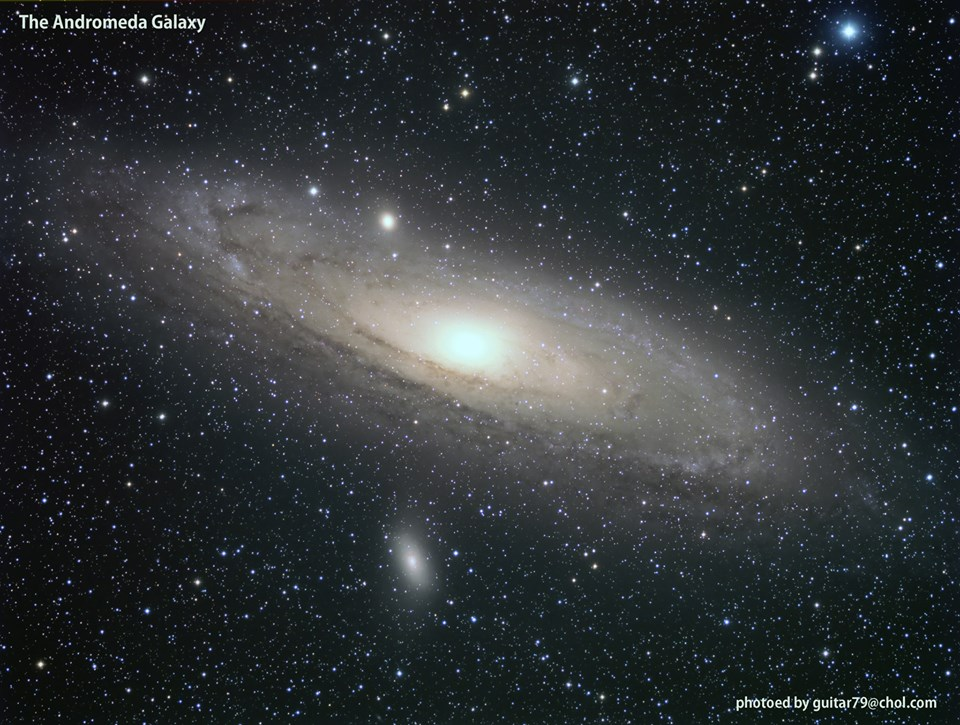
\includegraphics[width=0.7\linewidth]{Andromeda_Galaxy}
	\end{center}
		\caption{The Andromeda galaxy : L 600s X 14 frames, RGB 400s X 6 frames each (Takahashi FSQ106-ED with 0.73X Reducer QE, Sbig ST-8300M, Takahashi EM-200 Temma 2).}
		\label{fig:The_Andromeda_Galaxy}
\end{figure}

광학계에 의한 별의 상이 검출기에 정확하게 맺히도록 하기 위해서는 포커서(focuser)를 정밀하게 움직여야 한다. 사진 촬영을 위한 고성능의 광학계는 포커서를 견고하게 만들 뿐 아니라 포커서 노브에 미동 장치가 있어 정밀하게 초점 조절이 가능하다. 하지만 포커서를 조절하기 위해 손이 포커서에 닿을 경우 그 진동이 상에 영향을 미치기 때문에 이를 줄이기 위해 숙달이 필요하다.. 

또한 관측을 하는 동안 온도 변화에 의해서 망원경의 초점이 변하기도 한다. 이를 해결하기 위하여 Persha(2001)는 주위 온도에 따라 변하는 초점 보정하기 위한 온도 보상 초점 방법을 연구하였다 \cite{persha2001temperature}.


\subsection{연구 목적}

본 연구에서는 천체 망원경의 포커서를 손으로 조절할 경우에 생기는 진동으로 생기는 문제점을 해결하기 위하여 포커서에 스테핑 모터를 장착한 모터 포커서를 정밀하게 제어할 수 있는 모터 포커서 컨트롤러를 제작하여 실제 관측에 사용하는 것을 목적으로 한다. 

제작한 모터 포커서 컨트롤러는 GS-touch로 명명하였다. GS-touch는 스테핑 모터를 구동할 수 있고 컴퓨터로 제어할 수 있도록 설계하였다. 또한 전용 ASCOM(Astronomy Common Object Model) dirver를 개발하여 ASCOM을 지원하는 천문 소프트웨어를 이용하여 쉽게 사용할 수 있도록 하였다.

본 연구의 또 다른 목적은 관심있는 사람들은 직접 부품을 구입하여 제작할 수 있도록 제작 과정과 노하우를 공개하여 아이디어 나눔을 실천하는 것도 포함된다.


\subsection{연구 문제}

%% 박기현샘 : 연구문제의 답이 결론에 제시되어야 함. 둘이 호응관계가 되도록 기술
천체 망원경 모터 포커서 컨트롤러 개발과 관련된 본 연구에서 다루는 연구문제는 다음과 같다. 

1. 아두이노 나노를 기반으로 2상 바이폴라 스테핑 모터 드라이버, OLED 디스플레이어, 온습도 센서 등이 연결된 모터 포커서 컨트롤러인 GS-touch의 하드웨어를 제작할 수 있는가?

2. 제작한 GS-touch 모터 포커서 컨트롤러가 천체 망원경의 초점 조절을 수행할 수 있도록 펌웨어를 개발할 수 있는가?

3. 제작한 GS-touch 모터 포터서 컨트롤러가 자동 초점 조절 기능이 있는 MaximDL, FocusMAX 등의 소프트웨어로 구동될 수 있도록 ASCOM driver 개발할 수 있는가?